\section{Existing languages}
Before doing any work on the group's own language, it was decided to look into the high-level languages that already exist for the Arduino platform, and what distinguishes them from each other.
This was done in part to find out what kind of competition there may be for HCL, and in part to gain inspiration from the existing languages.
There is a variety of languages to choose from when programming for the Arduino.
Some of these are:

\begin{itemize}
	\item Arduino C++ (the official Arduino language)
	\item Occam-pi
	\item NanoVM
	\item Juniper
	\item ArduinoBlocks
\end{itemize}

% Source: arduino.cc
\textbf{Arduino C++} is a subset of the C++ language with its own libraries, designed specifically for the Arduino.
Because of this, it is compatible with the C and C++ languages.
There are a few changes made to the language, but the basic functionality and syntax of C and C++ are still present, meaning users are able to use both the imperative- and the object-oriented paradigms of C and C++ respectively to program the Arduino.

The following is a brief overview of the basic syntax of the Arduino C++.
Snippets \ref{lis:arduinoExample} and \ref{lis:arduinoHeader} show an example program showcasing the syntax.
All information is taken from the official Arduino reference\cite{ArduinoReference}.

The language requires two functions to be declared;
the \texttt{setup} function which is called at startup,
and the \texttt{loop} function with is called in an infinite loop after the \texttt{setup} code is run.

All \textit{statements} are finished with a semi-colon.

\textit{Variables} are declared by specifying a type and following it up with an identifier (snippet \ref{lis:arduinoExample}, line 11).
Declarations can be prefixed with the \texttt{const} keyword to make the variable immutable, or \texttt{static} to mark it as persistent between function calls.
All variables have to be initialized before they are used. 

\textit{Functions} are declared with a return type, a name, parameters enclosed in parentheses, and a body encapsulated with curly-brackets (snippet \ref{lis:arduinoExample}, line 29).
If the function does not return a value, the return type is set to \texttt{void}.
If it is a class function, the class must be specified in the declaration (snippet \ref{lis:arduinoExample}, line 22).

\textit{Classes} are declared with the keyword \texttt{class} followed by a name and the class body encapsulated in curly-brackets (snippet \ref{lis:arduinoHeader}, line 1).
The class' field is declared in the body, but isn't initialized here.
Similarly, functions aren't given bodies in the class declaration either.
Instead, the functions must be given a body outside of the class, and the variables must be initialized in the constructor function, also outside of the body.

\textit{Preprocessor directives} such as including a header file, or setting up macros are written with a pound symbol (snippet \ref{lis:arduinoExample}, lines 6-9).

\textit{Comments} can be written in two different ways.
The end-of-line comment is prefixed with two slashes (snippet \ref{lis:arduinoExample}, line 6).
The multi-line comment is prefixed with a slash followed by an asterisk (\texttt{"/*"}), and postfixed with an asterisk followed by a slash (\texttt{"*/"}) (snippet \ref{lis:arduinoExample}, line 1-4).

\begin{lstlisting}[language=C++,label=lis:arduinoExample,caption=An example program written in the Arduino language.,firstnumber=1]
/*
 * This program makes an LED connected to pin 13 on the arduino
 * board blink on and off every 500 milliseconds
 */

#include "Arduino.h" //The Arduino standard library
#include "Blinker.h" //The Blinker custom library

#define LED_PIN 13 //Symbolic constant

const int BLINK_DELAY = 250; //Constant, global integer variable

Blinker blinker(LED_PIN, BLINK_DELAY); //Object instantiation

void setup() {} //No setup code for this program

void loop()
{
    blinker.Blink(); //Program blinks infinitely
}

Blinker::Blinker(int pin, int msDelay)
{
	pinMode(pin, OUTPUT);
	_pin = pin;
	_msDelay = msDelay;
}

void Blinker::Blink()
{
	digitalWrite(_pin, HIGH);
	delay(_msDelay);
	digitalWrite(_pin, LOW);
	delay(_msDelay);
}

\end{lstlisting}

\begin{lstlisting}[language=C++,label=lis:arduinoHeader,caption=The Blinker.h header file.,firstnumber=1]
class Blinker
{
	public:
		Blinker(int pin, int msDelay); //Constructor
		void Blink();
	private:
		int _pin;
		int _msDelay;
};
\end{lstlisting}

% Source: concurrency.cc
\textbf{Occam-pi} is a language that focuses on making parallel programming easy for programmers.
It is based on Occam that first appeared in 1983.
The full documentation of Occam-pi can be read on the official website of the language, \url{concurrency.cc}, but following here is a short description of some of the syntax, and an example program in Snippet \ref{lis:occamExample}.

\textit{Variables} are declared by initializing them with the colon-equals operator (lines 6-7). 
Type is automatically inferred by the expression on the right hand side of the initializing assignment.

\textit{Functions} in Occam-pi are declared using the keyword \texttt{PROC} followed by a name and the function parameters enclosed in parentheses (line 5).
Unlike C, Occam-pi doesn't use curly-brackets to encapsulate the body.
Instead, the body is indented using a tab, similar to the Python language.
The end of the function is marked using a colon.
One of the key features of Occam-pi is the fact that it separates expressions that are evaluated sequentially and ones that are evaluated concurrently using the \texttt{SEQ} and \texttt{PAR} keywords.

\textit{Preprocessor directives} are, like in C, prefixed with a pound symbol (line 3).

\textit{Comments} are prefixed with two dashes (\texttt{"{-}{-}"}) (line 1).

\begin{lstlisting}[language=C,label=lis:occamExample,caption=An example program written in Occam-pi.,firstnumber=1]
--This program makes two 

#INCLUDE "plumbing.module" --Include module preprocessor directive

PROC main ()
	SEQ --Expressions are evaluated sequentially
		x := 4 + 3
		y := x * 5
	PAR --Expressions are evaluated concurrently
		blink(12, 1000) --A function from the plumbing module
		blink(13, 1000)
:
\end{lstlisting}

% Source: http://www.harbaum.org/till/nanovm/index.shtml
\textbf{NanoVM} is a virtual machine (VM) for the Atmel AVR ATMega8 CPU.
It allows programmers to write code in a subset of Java that can be run by Arduino and similar microcomputers.
The VM includes many of the features that have made the Java VM (JVM) popular such as object-oriented programming, automatic dynamic memory allocation, and garbage collection.
It comes packaged with native classes such as Object, System, and PrintStream.

The following is a short description of the basic Java syntax. 
Snippets \ref{lis:javaExample} and \ref{lis:javaPrinter} showcase the syntax.

The program is started by calling the \texttt{main} function (snippet \ref{lis:javaExample}, line 5).

All statements are finished with a semi-colon.

In Java all variables and functions must be declared inside a class, and each class must be declared in a file for itself.

\textit{Class fields} and methods are declared identically to how variables are declared in Arduino C++, except each field variable is prefixed with an optional access modifier (snippet \ref{lis:javaExample}, lines 3, 5).
Variables can be made into class variables (called so because the variables belong to the class instead of instances of the class) with the \texttt{static} keyword before the name in the declaration.
The same can be done to methods.

\textit{Comments} are written exactly like in C and C++.

\begin{lstlisting}[language=Java,label=lis:javaExample,caption=An example program written in Java.,firstnumber=1]
public class HelloWorld {

	private static Printer printer = new printer(); //Class variable
	
	public static void main(String[] args) { //Program start
		printer.print("Hello World!");
	}
	
}
\end{lstlisting}

\begin{lstlisting}[language=Java,label=lis:javaPrinter,caption=Printer class with one method written in Java.,firstnumber=1]
public class Printer {
	public void print(String str) { //Instance method
		System.out.println(str);
	}
}
\end{lstlisting}

The downsides of using NanoVM instead of Arduino C++ is, as stated on the official website of NanoVM\footnote{http://www.harbaum.org/till/nanovm/index.shtml} that the VM's interpreter doesn't perform as well as C compiled to AVR code, and it reserves some of the RAM used for applications to run the VM.
NanoVM also has to be installed on the CPU's flash memory, which will overwrite the bootloader.

\textbf{Juniper} is a functional programming language designed specifically for the Arduino.
The intention behind creating Juniper was to provide a higher level language than Arduino C++, which at the same time was more suited for programming electronic devices\cite{JuniperTutorial}.

The following is a description of the basic syntax of Juniper. 
Figure \ref{lis:juniperExample} showcases the syntax.

\textit{Variables} are declared using the \texttt{let} keyword followed by a name, an equal sign, and an expression (line 4).
Variables are by default immutable, ie. 
they can't be assigned another value after declaration, but they can be made mutable by inserting the \texttt{mutable} keyword before the name in their declaration.

\textit{Functions} are declared using the \texttt{fun} keyword followed by a name, parameters enclosed in parentheses, an equal sign, and the function body encapsulated in parentheses (line 9).

\textit{Modules} have the same purpose and functionality as they do in Occam-pi - to provide predefined functions to the programmer.

\textit{Comments} in Juniper can be written in two different ways.
End-of-line comments are prefixed with two slashes (just like C++ and Java).
Multi-line comments are prefixed with a start parenthesis followed by an asterisk (\texttt{"(*"}), and post fixed with an asterisk followed by an end parenthesis (\texttt{"*)"}).

\begin{lstlisting}[,label=lis:juniperExample,caption=Example program\, taken from the tutorial on Juniper's website.,firstnumber=1]
module Blink
open(Prelude, Io, Time)

let boardLed = 13

let tState = Time:state()
let ledState = ref low()

fun blink() = (
	let timerSig = Time:every(1000, tState);
	let ledSig =
		Signal:foldP(
			fn (currentTimer, lastState) ->
				Io:toggle(lastState)
			end,
			ledState, timerSig);
	Io:digOut(boardLed, ledSig)
)

fun setup() =
	Io:setPinMode(boardLed, Io:output())

fun main() = (
	setup();
	while true do
		blink()
	end
)
\end{lstlisting}

\textbf{ArduinoBlocks} is a drag and drop programming language, similar to the language Scratch, wherein the user writes programs by grouping "blocks" together to form functions.
It provides a simple graphical user-interface and functions for various add-on modules for the Arduino, and the user isn't required to write much when programming in ArduinoBlocks.

Figure \ref{fig:arduinoBlocks} shows how the programming interface for ArduinoBlocks looks.

\begin{figure}[H]
	\centering
	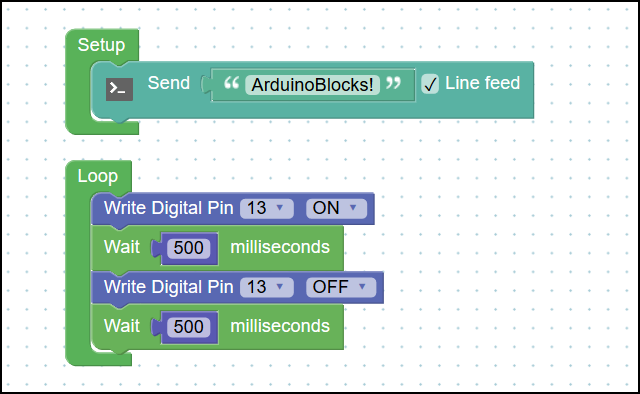
\includegraphics[width=\textwidth/2+\textwidth/4]{2.Analysis/images/ArduinoBlocks.png}
	\caption{The default code when opening ArduinoBlocks}
	\label{fig:arduinoBlocks}
\end{figure}

% Source: https://code.google.com/archive/p/dk-basic/
These are, of course, not all the available languages for programming for Arduino.
The project group is also aware of a language called DK-BASIC, a subset of BASIC designed to work on Arduino, but that language is still in its alpha stage, so it won't get more than a mention here.
